\section{Experimental Results}
\label{sec:experimental_results}
\subsection{Software Platform}
For our tests we are using \texttt{pandas},
a data manpilation librirary,
for reading data in structured formats such as
\texttt{.csv} and \texttt{.xlxs} files.
The AMIGOS dataset is avaible in \texttt{.mat} format.
As we would like to use Python for our work we used
the library \texttt{SciPi} to read this format in a Python friendly manner.
This library was also used for the signal processing portion of our project.
For ploting of figures we used \texttt{matplotlib.pyplot}.
For the various algorithms we used throughout this paper such as SVM we
used \texttt{sklearn}.
\begin{figure}[h]
    \centering
    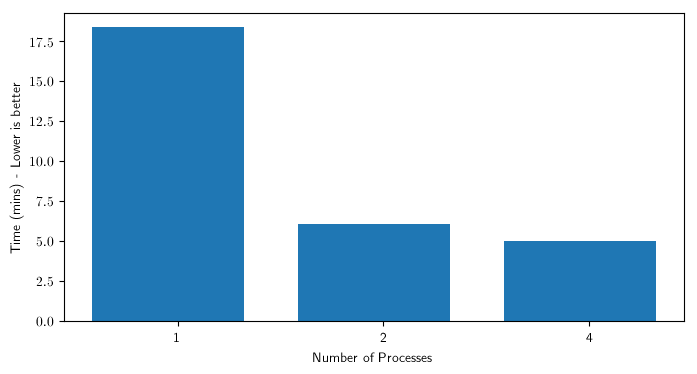
\includegraphics[width=\columnwidth]{tex/figures/multiprocess/multi_process_time.png}
    \caption{Time Taking to pre process data for different number of processes.}
    \label{fig:multip:time}
\end{figure}


\subsection{Performance of Multi-Process Feature Extraction}
On a 4 core Intel i5 processes we tested the performance of our feature extraction
for 1, 2, and 4 processes.
In Figure \ref{fig:multip:time} we can see the time taken to read and process
the data for these different process counts.
For a single process it took over 18 minuits to extract features.
There is only a minuit difference between the 2 and 4 process feature extraction phase.
That said we were able to get our time down to under 5mins.
This is around 3.6x improvemtn in performance.
While this does not improve our classification, this allowed us play
with our hyper parameters more frequently as each test took less time.
\begin{figure*}[h]
    \centering
    \begin{subfigure}[t]{\columnwidth}
        \centering
        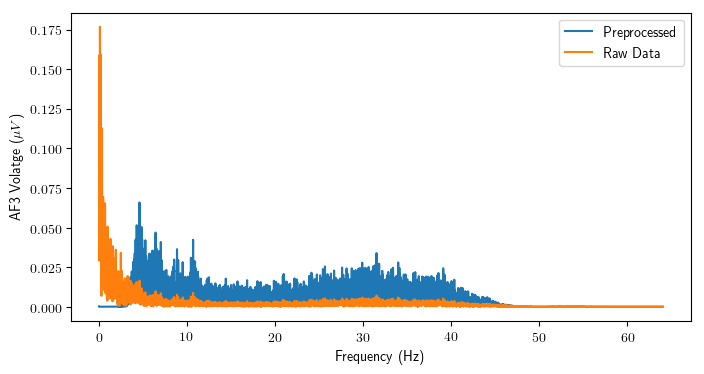
\includegraphics[width=\columnwidth]{tex/figures/filtering/AF3.png}
        \caption{AF3}
        \label{fig:filter:af3}
    \end{subfigure}
    \hfill
    \begin{subfigure}[t]{\columnwidth}
        \centering
        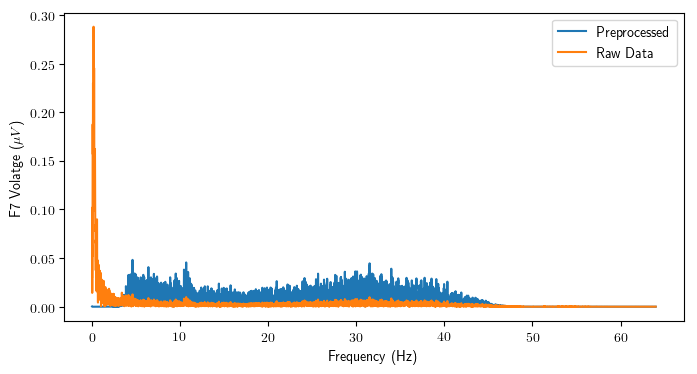
\includegraphics[width=\columnwidth]{tex/figures/filtering/F7.png}
        \caption{F7}
        \label{fig:filter:f7}
    \end{subfigure}
    \caption{Example filtering of EEG signal on sample 1 video 12}
    \label{fig:eeg}


    \begin{subfigure}[t]{\columnwidth}
        \centering
        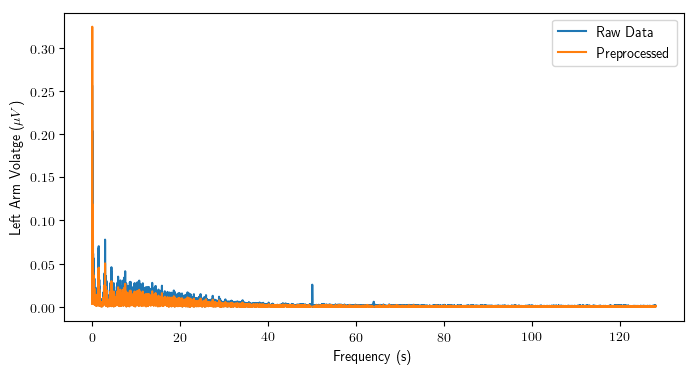
\includegraphics[width=\columnwidth]{tex/figures/filtering/ECG Left Arm.png}
        \caption{Left}
        \label{fig:filter:left}
    \end{subfigure}
    \hfill
    \begin{subfigure}[t]{\columnwidth}
        \centering
        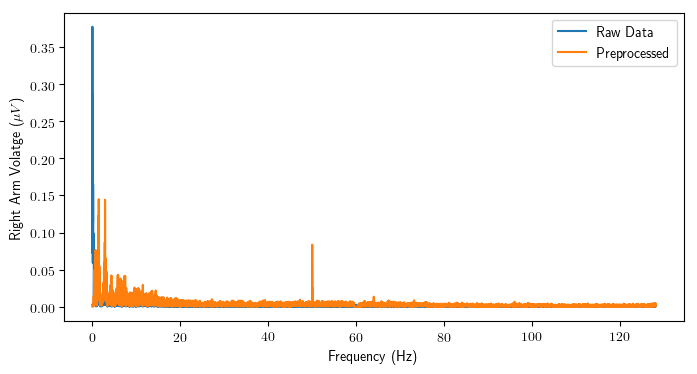
\includegraphics[width=\columnwidth]{tex/figures/filtering/ECG Right Arm.png}
        \caption{Right}
        \label{fig:filter:right}
    \end{subfigure}
    \caption{Example filtering of ECG signal on sample 1 video 12
             for the left and right arms}
    \label{fig:ecg}
\end{figure*}


\subsection{Preprocessing}
We have applied 3 processing steps to our AMIGOS dataset;
signal filtering, feature extraction, and dimentionality reduction.
In Figures \ref{fig:eeg} and \ref{fig:ecg}
we can see our filters applied to the EEG and ECG signals in the frequency domain.
For the EEG signal we followed the guideline set on the AMIGOS
website and applied a 4-45Hz bandpass filter \cite{AMIGOS:2018}.
We removed a significant amount of low frequency noise.
We can see that the preproccessed data results
in an slightly high amplitude than our original signal despite keeping the same shape.
Through experimental analysis we noticed that this was by a factor of 5.
For the ECG signal we applied a 0.05Hz highpass filter as noted in
\cite{SantamariaGranados:2019}
to remove baseline wander.
We also applied a bandstop filter with a 50Hz cutoff.
A small notch is visible in
Figures \ref{fig:ecg}.
The impact of the frequency filtering in the time domain can be seen in Figure
\label{fig:ecg:time}.

\subsection{Classification Results}
\begin{table}[h]
\caption{Logistic Regression}
\label{table:logistic}
\centering
\begin{tabular}{|c|c|c|}
\hline
\textbf{Emotion} &  \textbf{F1} &  \textbf{Accuracy} \\ \hline \hline
neutral & 0.685 & 0.713 \\ \hline
disgust & 0.889 & 0.900 \\ \hline
happiness & 0.858 & 0.8875 \\ \hline
surprise & 0.788 & 0.813 \\ \hline
anger & 0.487 & 0.538 \\ \hline
fear & 0.756 & 0.800 \\ \hline
sadness & 0.720 & 0.738 \\ \hline
\end{tabular}
\end{table}
\begin{table}[h]
\caption{SVM}
\label{table:svm}
\centering
\begin{tabular}{|c|c|c|}
\hline
\textbf{Emotion} &  \textbf{F1} &  \textbf{Accuracy} \\ \hline \hline
neutral& 0.678 & 0.713  \\ \hline
disgust& 0.889 & 0.900 \\ \hline
happiness& 0.871 & 0.913 \\ \hline
surprise& 0.811& 0.850 \\ \hline
anger& 0.457& 0.525 \\ \hline
fear& 0.775 & 0.838 \\ \hline
sadness& 0.747 & 0.763 \\ \hline
\end{tabular}
\end{table}
\begin{table}[h]
\caption{KNN}
\label{table:knn}
\centering
    \begin{tabular}{|c|c|c|c|}
\hline
\textbf{Emotion} &  \textbf{F1} &  \textbf{Accuracy} & \textbf{Best K}\\ \hline \hline
neutral& 0.712& 0.725& 5 \\ \hline
disgust& 0.916& 0.925& 2 \\ \hline
happiness& 0.871& 0.9125& 4 \\ \hline
surprise& 0.827& 0.875& 16 \\ \hline
anger& 0.559& 0.575& 1 \\ \hline
fear& 0.794& 0.8375& 4 \\ \hline
sadness& 0.864& 0.875& 2 \\ \hline
\end{tabular}
\end{table}
\begin{table}[h]
\caption{AdaBoost}
\label{table:adaboost}
\centering
    \begin{tabular}{|c|c|c|}
\hline
\textbf{Emotion} &  \textbf{F1} &  \textbf{Accuracy} \\ \hline \hline
neutral& 0.683& 0.688 \\ \hline
disgust& 0.901& 0.925 \\ \hline
happiness& 0.852& 0.875 \\ \hline
surprise& 0.875& 0.875 \\ \hline
anger& 0.718& 0.725 \\ \hline
fear& 0.782& 0.775 \\ \hline
sadness& 0.785& 0.788 \\ \hline
\end{tabular}
\end{table}
\begin{table}[h]
\caption{Voting}
\label{table:voting}
\centering
    \begin{tabular}{|c|c|c|}
\hline
\textbf{Emotion} &  \textbf{F1} &  \textbf{Accuracy} \\ \hline \hline
neutral& 0.685& 0.713 \\ \hline
disgust& 0.895& 0.913 \\ \hline
happiness& 0.871& 0.913 \\ \hline
surprise& 0.811& 0.850 \\ \hline
anger& 0.660& 0.688 \\ \hline
fear& 0.775& 0.838 \\ \hline
sadness& 0.842& 0.863 \\ \hline
\end{tabular}
\end{table}

In Tables \ref{table:logistic}, \ref{table:svm}, \ref{table:knn}, and \ref{table:voting}
we have the output of the different classification methods which we used.
With all three methods we that the F1 scores and the accuracy are very close.
The exact accuracy which we obtain differs between the emototions which we try and classify.
That said generally the KNN results are better than the SVM and the Logistic Regression.
This could be because its a better model or because it is over fitting.
To be certain of KNN's superiour classification.
